\documentclass{article}

% ==== Estilo NeurIPS ====================================================
% Usa o style file OFICIAL (neurips_2024.sty) se ele estiver presente nesta
% pasta; baixe-o do site da conferência e coloque aqui. Caso contrário, recai
% num preâmbulo que aproxima o layout NeurIPS (coluna única, 10pt, margens 1in).
\usepackage[utf8]{inputenc}
\usepackage[T1]{fontenc}
\IfFileExists{neurips_2024.sty}{%
  \usepackage[preprint]{neurips_2024}%
}{%
  \IfFileExists{neurips_2023.sty}{\usepackage[preprint]{neurips_2023}}{%
    \usepackage[margin=1in]{geometry}%
    \usepackage{times}%
    \usepackage{titlesec}%
    \titleformat{\section}{\normalfont\large\bfseries}{\thesection}{0.6em}{}%
    \titleformat{\subsection}{\normalfont\bfseries}{\thesubsection}{0.6em}{}%
    \setlength{\parskip}{0.4em}\setlength{\parindent}{0pt}%
  }%
}
\usepackage{microtype}
\usepackage{booktabs}
\usepackage{amsmath}
\usepackage{xcolor}
\usepackage{enumitem}
\usepackage{graphicx}
\usepackage{tikz}
\usetikzlibrary{positioning, arrows.meta, fit, backgrounds, calc}
\usepackage[hidelinks]{hyperref}

% ---- TikZ styles ----
\definecolor{cengine}{HTML}{F3ECD8}
\definecolor{cenv}{HTML}{D9EAD3}
\definecolor{ctrain}{HTML}{CFE2F3}
\definecolor{cout}{HTML}{F4CCCC}
\definecolor{chead}{HTML}{FFF2CC}
\tikzset{
  blk/.style={draw, rounded corners=2pt, align=center, font=\small,
              minimum height=8mm, inner sep=4pt},
  lyr/.style={draw, rounded corners=1pt, align=center, font=\footnotesize,
              minimum height=7mm, minimum width=20mm, fill=ctrain},
  io/.style={draw, align=center, font=\footnotesize, minimum height=7mm, fill=cengine},
  hd/.style={draw, rounded corners=1pt, align=center, font=\footnotesize,
             minimum height=7mm, fill=chead},
  fl/.style={-{Stealth[length=2mm]}, thick},
}

\title{\bfseries Reinforcement Learning in an Asymmetric, Perfect-Information
Historical Wargame: The Yom Kippur War}

\author{
  \emph{Yom Kippur Digital} project \\
  Digital reconstruction and reinforcement-learning study \\
  \texttt{github.com/.../yom-kippur-game}
}
\date{}

\begin{document}
\maketitle

\begin{abstract}
We present a complete reinforcement-learning (RL) case study on a historical
hex-and-counter wargame --- \emph{The Yom Kippur War} --- digitally reconstructed from
its original components (board, counters, and combat tables). The game has perfect
information with randomness confined to dice-based combat resolution (2d6), short
episodes (6 rounds, $\sim$90 micro-decisions per side), and strong \textbf{asymmetry}
between an attacker (Israel), who must chain a long-range amphibious operation, and a
defender (Egypt), which is reactive and locally advantaged. We build a vectorized
environment on the game's own rules engine, with a masked action space decomposed into
micro-decisions, and train PPO policies with three architectures: an MLP, a CNN over the
hexagonal grid and a GNN over the board's exact topology. An architecture-agnostic
interpreter serves them in the browser with verified numerical parity. The study then
adds PUCT search with a learned value, an AlphaZero-style loop and temporal abstraction
with an LLM strategist. Results on architecture--role fit and on the collapse of naive self-play
were measured against the heuristic opponent of the time and are reported as such.
\textbf{A later audit of the evaluation reverses the study's central negative claim.}
The heuristic opponent changed during the study and most comparisons rested on 12
games, so the apparent ceiling near 33\% for the attacker was an artifact. Retrained
against the current defender, the attacker wins 87\% instead of 14\%; adding the
heuristic's move to the candidates of PUCT raises search from 23.5\% to 55\%; and tuning
the heuristic's weights by the cross-entropy method nearly triples the heuristic
attacker. Every agent trained against a single opponent, however, is exploited by some
counter-strategy: the 87\% attacker loses all 1000 validation games to a reweighted
heuristic defender. \textbf{We therefore summarize the game by the Nash equilibrium of a
population} of eight attackers and six defenders after one PSRO iteration, in which the
attacker wins 17\%. We release the game, environment, trainer, search, evaluation arena
and models as a reproducible artifact.
\end{abstract}

\section{Introduction}

Board games have served for decades as testbeds for sequential decision-making.
Operational hexagonal wargames (\emph{hex-and-counter}), however, are comparatively
underexplored by RL despite attractive properties: discrete, well-defined rules; a
short horizon; and --- in the game studied here --- \textbf{structural asymmetry}
between the two sides, which exposes multi-agent RL difficulties that are rarely visible
in symmetric games such as Go or Chess.

We study \emph{The Yom Kippur War} (Wargame II), a simulation of the Israeli crossing of
the Suez Canal in October 1973. The Israeli general (attacker) has 6 rounds to destroy
surface-to-air (SAM) batteries, establish a bridgehead on the west bank, and control
city entrances; the Egyptian general (defender) seeks to prevent this. The historical
operation was notably audacious precisely because the position favored the defender ---
an asymmetry that is mirrored in the RL dynamics.

\textbf{Contributions.}
\begin{enumerate}[leftmargin=1.4em,itemsep=2pt]
  \item An \textbf{RL environment faithful to the production rules engine} (the same
  code that runs the playable game), eliminating train/deployment divergence.
  \item A \textbf{micro-decision action space with a legality mask} derived from the
  engine itself, making a combinatorial turn (moving up to 19 units) tractable.
  \item An \textbf{architecture-agnostic layer interpreter} that lets us train MLP/CNN/GNN
  in PyTorch and serve any of them in pure JavaScript in the browser, with tested
  numerical parity.
  \item An \textbf{AlphaZero-style PUCT search with a learned value} (opponent and chance
  folded into the transition, leaves scored by the PPO critic) and a complete self-play
  retraining loop, both runnable in the browser/Node from the same exported networks.
  \item Empirical findings on \textbf{architecture$\leftrightarrow$role fit},
  \textbf{self-play collapse in asymmetric games} and its \textbf{partial mitigation}.
  \item An \textbf{audit of the evaluation} (Section~\ref{sec:revisit}): a parallel arena
  with Wilson intervals, the finding that the opponent changed mid-study, retraining and
  cross-entropy tuning of both sides, a candidate-set fix for search, and a
  \textbf{population Nash} after one PSRO iteration as the summary of the game.
\end{enumerate}

\section{Related Work}

Tree-search self-play methods (AlphaZero and successors) reached super-human performance
on symmetric perfect-information board games. PPO is an established, robust baseline for
policy-based control. In multi-agent RL, naive self-play is known to be unstable
(non-transitive cycles, catastrophic forgetting), motivating opponent leagues and
\emph{fictitious play}. Potential-based reward shaping provides dense signal without
changing the optimal policy. KL penalties against a reference policy are used to limit
drift and preserve knowledge. Our work proposes no new algorithm; it combines known
techniques in an underexplored asymmetric domain and documents the resulting phenomena,
with an emphasis on reproducibility and deployment.

\section{The Game as an RL Environment}

\subsection{Domain}
The board is a hexagonal grid of \textbf{538 valid cells} (columns 1--25, rows 1--22;
flat-top topology with even columns shifted), with \textbf{1521 adjacency edges}. Seven
terrain types modulate movement cost and defensive bonus; roads, the Suez Canal, and a
freshwater canal are edge features. Each side controls battalions with a Combat Index
(CI) and a Mobility Index (MI); units take casualties (flip to a reduced-value back) and
are eliminated on the second casualty.

A round has \textbf{8 phases} (movement, attack declaration, defensive support, and
resolution --- first for Israel, then for Egypt). Combat between adjacent units is
\textbf{mandatory}; the outcome follows the force ratio (with terrain) mapped to a column
($-2$ to $+2$) of an Effects Table read with 2d6. The only source of randomness is this
roll. Victory conditions are asymmetric and graded (decisive/partial/marginal) per side.

\begin{figure}[t]
\centering
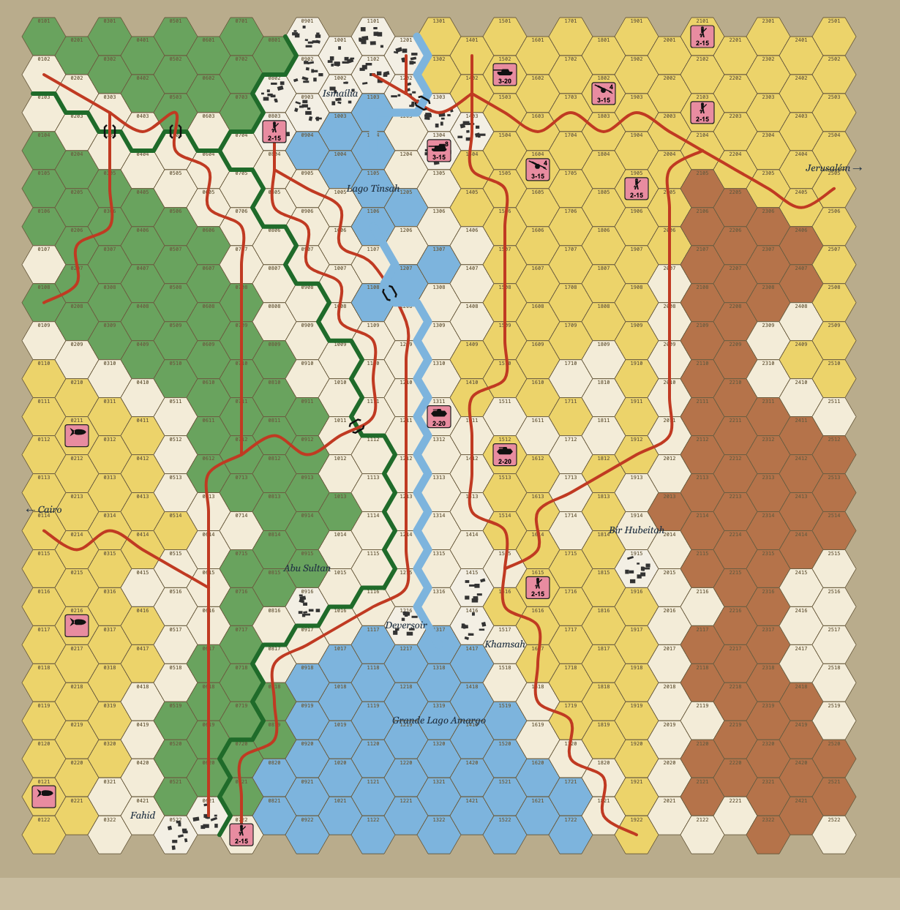
\includegraphics[width=0.62\linewidth]{board.png}
\caption{The reconstructed board (digital rendering of the original map sheet no.~4).
The Suez Canal and lakes run vertically in blue; the freshwater canal threads in dark
green; the road network in red. Forest (west), open, dunes (east), and rough (far east)
terrain are color-coded. Pink and blue counters are the initial Egyptian and Israeli
forces; the Israeli attacker enters from the east and must cross the canal toward the
SAM batteries and city entrances on the west bank.}
\label{fig:board}
\end{figure}

\subsection{MDP formulation}
\begin{itemize}[leftmargin=1.4em,itemsep=2pt]
  \item \textbf{Episode:} one game (6 rounds).
  \item \textbf{Decision (step):} one micro-decision --- a unit's destination, a
  reinforcement's entry cell, or an artillery support target.
  \item \textbf{Action:} an integer in $\{0,\dots,537\}$ (cell index) $\cup$ \{PASS\},
  totaling \textbf{539} actions. The cell's semantics depend on the current decision.
  \item \textbf{Mask:} a binary vector of legal actions, taken directly from the engine;
  the policy never explores illegal moves.
  \item \textbf{Observation:} 20 planes of 538 cells (one-hot terrain, roads, bank,
  objectives, SAMs; per side: presence, CI, MI, casualties, artillery-ready) $+$ 8
  scalars, totaling 10{,}776 values, \textbf{relative to the deciding side}.
  \item \textbf{Reward:} terminal, graded --- decisive $\pm1.0$, partial $\pm0.6$,
  marginal $\pm0.3$, draw 0; $\gamma=1$ given the short horizon.
\end{itemize}
Tactically minor choices during resolution (which unit takes a casualty, retreat
direction) are delegated to a heuristic, keeping the action space focused on strategic
decisions.

\subsection{System architecture}
The rules engine (JavaScript) is shared between the playable game and training. A Node
process exposes $K$ vectorized environments (JSON-lines protocol, base64 observations); a
Python trainer drives $M$ processes $\times\,K$ environments in lockstep ($\sim$700--1700
decisions/s on a 14-core CPU). Reusing the production engine guarantees that the policy
sees in training exactly what it will see when playing (Fig.~\ref{fig:system}).

\begin{figure}[t]
\centering
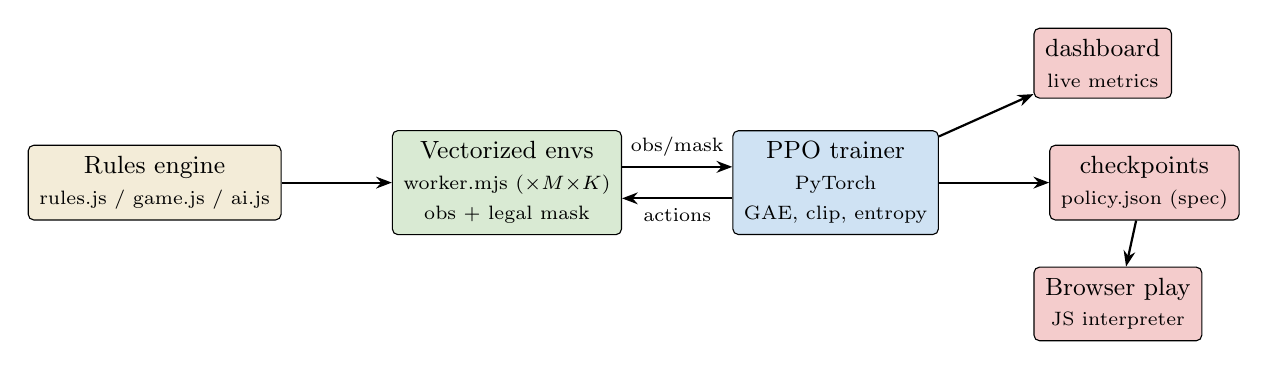
\begin{tikzpicture}[node distance=10mm and 14mm]
  \node[blk, fill=cengine] (eng) {Rules engine\\\scriptsize rules.js / game.js / ai.js};
  \node[blk, fill=cenv, right=of eng] (env) {Vectorized envs\\\scriptsize worker.mjs ($\times M{\times}K$)\\\scriptsize obs + legal mask};
  \node[blk, fill=ctrain, right=of env] (tr) {PPO trainer\\\scriptsize PyTorch\\\scriptsize GAE, clip, entropy};
  \node[blk, fill=cout, above right=4mm and 12mm of tr] (dash) {dashboard\\\scriptsize live metrics};
  \node[blk, fill=cout, right=of tr] (ckpt) {checkpoints\\\scriptsize policy.json (spec)};
  \node[blk, fill=cout, below right=4mm and 12mm of tr] (br) {Browser play\\\scriptsize JS interpreter};
  \draw[fl] (eng) -- (env);
  \draw[fl] ([yshift=2mm]env.east) -- node[above,font=\scriptsize]{obs/mask} ([yshift=2mm]tr.west);
  \draw[fl] ([yshift=-2mm]tr.west) -- node[below,font=\scriptsize]{actions} ([yshift=-2mm]env.east);
  \draw[fl] (tr) -- (dash);
  \draw[fl] (tr) -- (ckpt);
  \draw[fl] (ckpt) -- (br);
\end{tikzpicture}
\caption{System pipeline. The same rules engine backs both the playable game and the
vectorized training environments; trained policies are exported as an
architecture-agnostic layer spec and served in-browser by a pure-JS interpreter.}
\label{fig:system}
\end{figure}

\section{Method}

\subsection{Heuristic baseline and policy definitions}
\label{sec:heur}
The fixed opponent used for curricula and as an evaluation yardstick is a
\textbf{greedy, 1-ply heuristic} (no search, no learning) that plays either side
through the same rules engine. It is organized as a per-phase dispatcher.

\textbf{Doctrine via target lists.} High-level behavior emerges from per-unit target
sets rather than a planner. For Israel: the engineer seeks the best bridge-eligible
cell (east bank, between the lakes, far from enemies); before the bridge is up the
maneuver units escort/rescue it; afterwards their targets become the uncontrolled
victory objectives (Ismailia/Fahid entrances, live SAM cells). For Egypt: units already
on a defensive objective garrison it; if the Israeli bridge is up, the engineer becomes
the army's priority target (destroying it removes the bridge and cuts reinforcements);
otherwise units spread between objectives and containment.

\textbf{Position scoring.} In the movement phase, the heuristic enumerates a unit's
reachable cells (from the engine's terrain-/ZOC-aware Dijkstra) and picks the
$\arg\max$ of a hand-crafted scalar score. For a candidate cell $c$ and unit $u$,
\[
\text{score}(u,c) \;=\; -10\,d(c,\mathcal{T}_u)\;+\;80\,\mathbf{1}[c\in\mathcal{T}_u]
\;+\;\rho\big(\kappa(u,c)\big)\;+\;2\,b(c)\;-\;\xi(u,c),
\]
where $d(c,\mathcal{T}_u)$ is the hex distance to the nearest target in the unit's
target set $\mathcal{T}_u$; $b(c)$ is the terrain defensive bonus; and $\xi$ penalizes
\emph{exposure} (much more enemy than friendly Combat Index within radius~3). The
dominant term $\rho(\kappa)$ reflects that combat is \emph{mandatory}: ending adjacent
to an enemy commits the unit to attack next phase, so the heuristic estimates the
resulting Combat-Results-Table column $\kappa$ and scores
\[
\rho(\kappa)=\begin{cases}
+70 & \kappa\ge +2 \quad(\text{triple-odds attack, no elimination risk})\\
+35 & \kappa=+1\\
-25 & \kappa=\;\text{``=''}\quad(\text{eliminates the attacker on high rolls})\\
-100 & \kappa<0,
\end{cases}
\]
with an extra $-80$ for artillery/engineer (support units should not engage). The
\textbf{column estimate} $\kappa(u,c)$ simulates the combined combat the move would
trigger: it sums the Combat Index of the moving unit with that of all friendly units
already adjacent to the affected enemies (which the rules fuse into a single combat),
adds each defender's terrain bonus, and maps the resulting force ratio to a column in
$\{-2,\dots,+2\}$. Artillery barrage/cover is allocated only when it \emph{improves}
that column (each battery fires once per round); resolution-time choices sacrifice the
weakest/wounded unit and retreat so as to maximize distance from the enemy.

\textbf{Two scoring modes.} The fixed weights $\rho(\kappa)$ were in use when the
curricula of Section~\ref{sec:archfit} were trained. A later variant replaces $\rho$ by
the expected utility of the combat, $65\,\mathrm{E}_{2d6}[U(\kappa)]$, where $U$ assigns
a utility to each outcome of the Combat Results Table and the expectation runs over the
2d6 distribution. This \emph{expectimax} mode became the default for both sides and is
the opponent in every evaluation from Section~\ref{sec:puctres} onward. As
Section~\ref{sec:moving} shows, the change is far from neutral: it strengthens the
defender considerably and weakens the attacker.

\textbf{Policy definitions.} A neural policy defines
$\pi_\theta(a\mid s)=\mathrm{softmax}\big(\text{mask}(z_\theta(s))\big)$, where
$z_\theta$ are the per-action logits and $\text{mask}(\cdot)$ sets illegal actions to
$-\infty$; we sample $a\sim\pi_\theta$ during training (for exploration) and take
$\arg\max_a \pi_\theta$ at evaluation (greedy). The heuristic policy is the
deterministic $\arg\max$ of $\text{score}(u,\cdot)$ above. Both expose the identical
interface $\texttt{playPhase}(s)$ over the engine, so any side of any game can be driven
by either a network, the heuristic, or a human, interchangeably --- which is what lets
the same trained policy serve as a curriculum opponent, a league member, and an
in-browser AI.

\subsection{Architectures}
Three policies with the common interface $(\text{obs}, \text{mask}) \to
(\text{logits}[539], \text{value})$. The trunk differs; both heads are shared in spirit:
a \emph{policy head} emits one logit per cell plus a PASS logit, and a \emph{value head}
maps a global pooling (concatenated with scalars) to a scalar. The mask adds $-\infty$ to
illegal logits before the softmax. Figure~\ref{fig:nets} details the three trunks.

\begin{figure}[t]
\centering
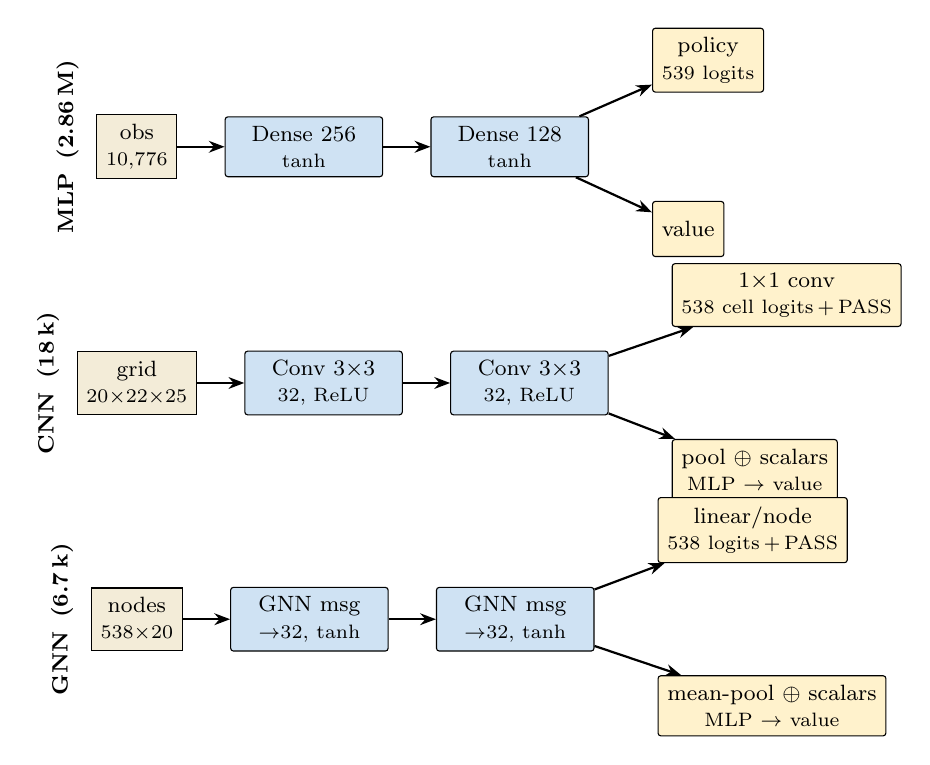
\begin{tikzpicture}[node distance=6mm]
  % ---------- MLP ----------
  \begin{scope}
    \node[io] (mi) {obs\\\scriptsize 10{,}776};
    \node[lyr, right=of mi] (m1) {Dense 256\\\scriptsize tanh};
    \node[lyr, right=of m1] (m2) {Dense 128\\\scriptsize tanh};
    \node[hd, above right=3mm and 8mm of m2] (mp) {policy\\\scriptsize 539 logits};
    \node[hd, below right=3mm and 8mm of m2] (mv) {value};
    \draw[fl] (mi)--(m1); \draw[fl] (m1)--(m2); \draw[fl] (m2)--(mp); \draw[fl] (m2)--(mv);
    \node[left=1mm of mi, font=\bfseries\footnotesize, rotate=90, anchor=south] {MLP\, (2.86\,M)};
  \end{scope}
  % ---------- CNN ----------
  \begin{scope}[yshift=-30mm]
    \node[io] (ci) {grid\\\scriptsize $20{\times}22{\times}25$};
    \node[lyr, right=of ci] (c1) {Conv $3{\times}3$\\\scriptsize 32, ReLU};
    \node[lyr, right=of c1] (c2) {Conv $3{\times}3$\\\scriptsize 32, ReLU};
    \node[hd, above right=3mm and 8mm of c2] (cp) {$1{\times}1$ conv\\\scriptsize 538 cell logits\,+\,PASS};
    \node[hd, below right=3mm and 8mm of c2] (cv) {pool $\oplus$ scalars\\\scriptsize MLP $\to$ value};
    \draw[fl] (ci)--(c1); \draw[fl] (c1)--(c2); \draw[fl] (c2)--(cp); \draw[fl] (c2)--(cv);
    \node[left=1mm of ci, font=\bfseries\footnotesize, rotate=90, anchor=south] {CNN\, (18\,k)};
  \end{scope}
  % ---------- GNN ----------
  \begin{scope}[yshift=-60mm]
    \node[io] (gi) {nodes\\\scriptsize $538{\times}20$};
    \node[lyr, right=of gi] (g1) {GNN msg\\\scriptsize $\to$32, tanh};
    \node[lyr, right=of g1] (g2) {GNN msg\\\scriptsize $\to$32, tanh};
    \node[hd, above right=3mm and 8mm of g2] (gp) {linear/node\\\scriptsize 538 logits\,+\,PASS};
    \node[hd, below right=3mm and 8mm of g2] (gv) {mean-pool $\oplus$ scalars\\\scriptsize MLP $\to$ value};
    \draw[fl] (gi)--(g1); \draw[fl] (g1)--(g2); \draw[fl] (g2)--(gp); \draw[fl] (g2)--(gv);
    \node[left=1mm of gi, font=\bfseries\footnotesize, rotate=90, anchor=south] {GNN\, (6.7\,k)};
  \end{scope}
\end{tikzpicture}
\caption{The three policy/value trunks. The MLP treats the observation as a flat vector;
the CNN convolves over the offset hex grid (each cell scattered to a $22{\times}25$
lattice); the GNN performs message passing over the exact 1521-edge hex adjacency. CNN
and GNN share weights across space and are two to three orders of magnitude smaller than
the MLP. ``GNN msg'' concatenates each node's features with the mean of its neighbors.}
\label{fig:nets}
\end{figure}

\subsection{Training (PPO) and deployment}
\label{sec:train}
We train with PPO using advantage estimated against a value baseline, clipping, and an
entropy bonus. Policies are exported as a \textbf{list of executable layers}
(\texttt{linear}, \texttt{conv}, \texttt{gnn}, heads), interpreted both by training and by
a pure-JavaScript inference engine --- enabling play against any architecture in the
browser with no dependencies. A parity test confirms that the interpreter's 539 logits
match PyTorch (max error $< 10^{-8}$).

\subsection{Self-play and stabilization}
In self-play both sides are policies in training, with a \textbf{league} of frozen
checkpoints (\emph{fictitious play}) and per-trajectory credit ($\gamma=1$). To curb the
attacker's degradation (Section~\ref{sec:collapse}), we combine:
\begin{itemize}[leftmargin=1.4em,itemsep=2pt]
  \item \textbf{Potential-based shaping:} $\Phi(s)$ grows with attacker progress (bridge,
  SAMs, objectives, bridgehead). With $\gamma=1$ the return telescopes to
  $R_{\text{terminal}} + \alpha\,(\Phi_{\text{final}} - \Phi_t)$, preserving the optimum
  (Ng et al., 1999).
  \item \textbf{Asymmetric self-play:} more epochs, learning rate, and fraction of
  environments for the weak side.
  \item \textbf{KL penalty against an anchor:} $\beta\,\mathrm{KL}(\pi_{\text{cur}}\,\|\,
  \pi_{\text{anchor}})$, the anchor being the attacker's curriculum policy.
\end{itemize}

\subsection{Search at inference: PUCT with a learned value}
\label{sec:puct}
At play time we optionally replace greedy policy evaluation with an AlphaZero-style
Monte-Carlo tree search, exploiting two structural simplifications of the domain. First,
because combat is mandatory and the opponent's phases and the 2d6 Effects Table are part
of the environment, we \textbf{fold the opponent and chance into the transition}: between
two of our movement decisions the heuristic plays the opponent's round and the engine
resolves combat (using the expectimax column choice of Section~\ref{sec:heur}). The tree
then contains only \emph{our} decision nodes, the value is always from our perspective,
and no minimax sign-flipping is needed --- a single-agent search against a fixed world
model. Second, we \textbf{never roll out to the end}: leaves are scored by the network's
value head $V_\theta$, the PPO critic trained to predict the graded terminal outcome,
which supplies the long horizon a $1$-ply policy lacks. Selection uses PUCT,
\[
a^\star=\arg\max_a\; Q(a)\;+\;c_{\text{puct}}\,P(a)\,\frac{\sqrt{\sum_b N(b)}}{1+N(a)},
\]
with prior $P$ the masked, top-$k$ policy head and $Q$ the mean backed-up leaf value; the
chosen move is the most-visited root action. Only the movement phase is branched; combat
phases use the base policy. Defaults: $c_{\text{puct}}{=}1.5$, $k{=}6$, $48$ simulations,
depth $4$ of our rounds. The value head, already exported with every network, is surfaced
to the JS interpreter; the parity test of Section~\ref{sec:train} is extended to confirm
both logits \emph{and} value match PyTorch to $<10^{-8}$.

\paragraph{AlphaZero refinement.} We further close the learning loop: PUCT self-play
generates targets $(\pi,z)$, where $\pi$ is the root visit distribution (with root
Dirichlet noise and an early-move temperature schedule for exploration) and $z$ the graded
outcome, on which we retrain the policy (cross-entropy to $\pi$) and value (MSE to $z$),
warm-started from the PPO models, and iterate. We also study a \emph{value-only} variant
that freezes the policy and refits only $V_\theta$, motivated by the result below.

\section{Experimental Setup}
Phase-A curricula train each side against a fixed heuristic AI for 150--200 updates (32
parallel environments). Evaluation is greedy, over 24--100 games with held-out seeds,
reporting win rate by type. For self-play, we seed the policies with the best curricula.
Main hyperparameters: lr $3\cdot10^{-4}$ (curriculum), clip $0.2$,
$\lambda_{\text{GAE}}\,0.95$, entropy $0.01$--$0.03$. Fixed seeds make games reproducible.

\textbf{Two evaluation protocols.} Section~\ref{sec:archfit} through
Section~\ref{sec:hier} report the protocol used when those experiments were run: greedy
play over 12 to 100 games, against the heuristic in whichever scoring mode was current.
Section~\ref{sec:revisit} re-evaluates with a parallel arena that plays complete games
across workers, reports Wilson 95\% intervals~\cite{wilson}, and uses at least 300 games
per condition and 1000 to validate optimized agents, always on seeds that were not seen
during training or tuning. Where the two disagree, the second should be preferred.

\section{Results}

\subsection{Architecture$\leftrightarrow$role fit (vs.\ heuristic)}
\label{sec:archfit}
\begin{center}
\begin{tabular}{lccc}
\toprule
\textbf{Side} & \textbf{MLP (2.86\,M)} & \textbf{CNN (18\,k)} & \textbf{GNN (6.7\,k)} \\
\midrule
Egypt (defender; reactive, local) & 100\% & --- & \textbf{92\%} \\
Israel (attacker; long-range plan) & \textbf{97\%} & 0\% & 0\% \\
\bottomrule
\end{tabular}
\end{center}

The Egyptian side, defensive and locally decided, is comfortably solved by small,
spatially structured networks --- the GNN reaches 92\% with 400$\times$ fewer parameters
than the MLP ($\sim$35\,KB vs.\ $\sim$15\,MB model). The Israeli side, which must chain
bridge $\to$ crossing $\to$ capture of scattered objectives, \textbf{is mastered only by
the high-capacity MLP}; CNN and GNN converge prematurely (entropy $\to 0$ around update
100) to a local optimum of ``losing by a smaller margin'' (reward $\sim-0.6$), never
winning. Section~\ref{sec:capacity} traces this specifically to \emph{capacity} (a wider
spatial net does win), not to an inductive-bias mismatch as one might first assume.
These rates were measured against the fixed-weight heuristic. Against the expectimax
defender used in later sections, the same attacker MLP wins 14.0\%
(Section~\ref{sec:moving}).

\subsection{Naive self-play collapse}
\label{sec:collapse}
Starting from the curriculum policies (ISR 97\%, EGY 92--100\% vs.\ heuristic), unmitigated
self-play \textbf{monotonically degrades the attacker}: its rate vs.\ the heuristic falls
from 97\% to 0\% and the head-to-head ISR$\times$EGY sits at $\sim$0. The structurally
favored defender wins almost always; with no positive reward signal, the attacker's
gradient drives it away from any prior competence (catastrophic forgetting).

\subsection{Stabilization}
We combine potential-based shaping, asymmetric self-play, and a KL anchor against the
attacker's curriculum policy. Table~\ref{tab:stab} compares naive self-play with two
mitigation settings: a moderate one ($\alpha{=}0.1$, $\beta{=}0.05$, 200 updates) and an
aggressive one ($\alpha{=}0.15$, $\beta{=}0.10$, $8$/$2$ epochs and $70\%$ of
environments for the attacker, 250 updates).

\begin{table}[t]
\centering
\caption{Self-play stabilization. ISR-vs-heuristic ``$=1$ rate'' is the fraction of
greedy evaluations in which the attacker still wins 100\% against the heuristic --- a
proxy for not having forgotten its curriculum competence. Head-to-head is the
attacker's win rate against the co-trained defender.}
\label{tab:stab}
\begin{tabular}{lccc}
\toprule
& \textbf{Naive} & \textbf{Mitigated ($\beta{=}0.05$)} & \textbf{Aggressive ($\beta{=}0.10$)} \\
\midrule
ISR vs.\ heuristic (mean) & $\to 0$ (stuck) & oscillates, recovers & \textbf{0.83} \\
ISR vs.\ heuristic ($=1$ rate) & 0 & --- & \textbf{28/50} \\
ISR$\times$EGY head-to-head (peak) & $\sim 0$ & 0.58 & 0.54 \\
ISR$\times$EGY head-to-head (mean) & $\sim 0$ & --- & 0.24 \\
EGY vs.\ heuristic & strong & strong & 0.71--0.96 \\
$\mathrm{KL}(\pi\,\|\,\text{anchor})$ & --- & $\le 0.39$ & 0.10--0.22 \\
\bottomrule
\end{tabular}
\end{table}

The mitigations \textbf{prevent the permanent collapse} of the naive case (where the
attacker is stuck at 0\%): the KL penalty re-anchors the policy whenever it degrades, so
the attacker spends most of training at 100\% vs.\ the heuristic (mean $0.83$; perfect in
$28$ of $50$ evaluations) and gains real head-to-head competitiveness (recurring peaks of
$0.46$--$0.54$, against $\sim$0 for naive self-play). The aggressive setting is the more
stable of the two. \textbf{Full balance is not reached}, however: the head-to-head mean
stays below $0.5$ because the defender is structurally favored. The techniques solve the
stated problem (avoiding collapse) but do not make the game symmetric --- a limit of the
domain, not of the method.

\subsection{Search strengthens the attacker; the value dominates the prior}
\label{sec:puctres}
We now add inference-time search (Section~\ref{sec:puct}). Table~\ref{tab:puct} compares,
apples-to-apples (same $12$ held-out seeds, same full game loop), the heuristic, the
greedy neural policy, and PUCT. This protocol is stricter than the curricula of
Section~\ref{sec:archfit}: absolute rates are lower because the seed set strongly favors
the defender (heuristic-vs-heuristic gives ISR $8\%$ / EGY $92\%$); the \emph{relative}
ordering is the point. \textbf{PUCT quadruples the attacker} ($8\%\!\to\!33\%$) and doubles
the greedy policy ($17\%\!\to\!33\%$): the value head delivers the strategic horizon the
$1$-ply policy lacks (it now ``sees'' the payoff of bridge $\to$ crossing $\to$ capture).
The defender, already near its heuristic ceiling ($92\%$), is not improved (PUCT and greedy
both $67\%$): search cannot exceed an evaluator that is itself weaker than the heuristic on
defense.

\emph{Note added in revision.} The explanation of the low absolute rates given above is
incorrect. They reflect a change of opponent, the expectimax defender of
Section~\ref{sec:moving}, rather than the seed set. On 300 games the heuristic baseline
is 15.3\%, not 8\%, and with 12 games each rate in Table~\ref{tab:puct} carries a 95\%
interval of about $\pm$25 points.

\begin{table}[t]
\centering
\caption{Inference-time search vs.\ greedy play and the heuristic (full game loop, $12$
defender-favoring held-out seeds, win rate vs.\ the heuristic). PUCT uses $48$ simulations.}
\label{tab:puct}
\begin{tabular}{lccc}
\toprule
\textbf{Side} & \textbf{Heuristic} & \textbf{Greedy policy} & \textbf{PUCT ($48$ sims)} \\
\midrule
Israel (attacker) & 8\% & 17\% & \textbf{33\%} \\
Egypt (defender)  & \textbf{92\%} & 67\% & 67\% \\
\bottomrule
\end{tabular}
\end{table}

A control isolates \emph{what} the search relies on. Driving PUCT with a \emph{stronger}
policy prior but a worse-calibrated value --- the $97\%$ curriculum MLP, whose critic only
ever saw heuristic play --- \emph{lowers} the attacker to $17\%$, below the $33\%$ obtained
from the self-play model's weaker policy but better-calibrated critic. \textbf{In PUCT here
the value dominates the prior}: search quality tracks the evaluator, not the actor. This
single observation governs all of the AlphaZero results that follow.

\paragraph{AlphaZero refinement: an instructive asymmetry.}
Table~\ref{tab:az} reports three controlled variants of the loop (Section~\ref{sec:puct},
$10$ seeds). \emph{(i)} Naive joint retraining \textbf{degrades} both sides: the sharp PPO
prior collapses toward the near-uniform $\pi$ produced by a low-simulation search.
\emph{(ii)} Freezing the policy and refitting \emph{only} the value isolates the cause ---
with the prior intact, the \textbf{defender improves ($70\!\to\!80\%$)} because its
self-play outcomes are informative, but the \textbf{attacker collapses to $0\%$}: in
defender-dominated self-play almost every attacker record is a loss ($z<0$), so its value
head loses the ability to \emph{discriminate} good positions from bad. \emph{(iii)}
Regenerating the attacker's targets against the heuristic (balanced, $\sim$$42\%$ wins)
recovers only part of the gap ($0\!\to\!10\%$, still below the $30\%$ PPO baseline): raw
Monte-Carlo targets from $24$ games are noisier than the PPO critic (trained with
bootstrapping over thousands of games), and the narrow-margin attacker is sensitive to
value variance. Surpassing the PPO value via AlphaZero would require large-scale data and
bootstrapped value targets, infeasible at $\sim$$10$\,s per searched game on one machine.
The pipeline is released ready to scale.

\begin{table}[t]
\centering
\caption{AlphaZero refinement (win rate vs.\ heuristic, $10$ held-out seeds), warm-started
from the PPO models. The value-only variant freezes the policy and refits only $V_\theta$.}
\label{tab:az}
\begin{tabular}{lcc}
\toprule
\textbf{Variant} & \textbf{Israel} & \textbf{Egypt} \\
\midrule
Baseline (PUCT, PPO value)        & 30\% & 70\% \\
Naive AZ (policy $+$ value)       & 0\%  & 60\% \\
Value-only, lopsided self-play    & 0\%  & \textbf{80\%} \\
Value-only, balanced targets      & 10\% & --- \\
\bottomrule
\end{tabular}
\end{table}

\subsection{Revisiting the small-network attacker: capacity, not inductive bias}
\label{sec:capacity}
Section~\ref{sec:archfit} left open \emph{why} only the high-capacity MLP masters the
attacker while the CNN/GNN converge to a ``lose-by-less'' optimum (reward $\sim-0.6$,
$0\%$ wins). A natural reading is an inductive-bias mismatch (translation-equivariant
weight sharing cannot pinpoint the single bridge cell or named objectives). A controlled
ablation \textbf{refutes} that explanation. Curriculum training is sparse-reward
(graded terminal only); we first add the potential-based shaping of
Section~\ref{sec:puct} ($\Phi$: bridge, SAMs, objectives, bridgehead) to the attacker's
curriculum, then vary network width (Table~\ref{tab:cap}). Shaping alone does \emph{not}
help a small net: the CNN/GNN never make partial progress, so $\Phi$ stays $\approx 0$ and
the shaping term is inert ($0\%$, identical to unshaped). But a \textbf{$7\times$ wider
GNN} (47.7\,k vs.\ 6.7\,k parameters) under the \emph{same} shaped settings \emph{learns
to win}, peaking at $33\%$ --- on par with the MLP under this protocol --- while the
narrow GNN with identical shaping stays at $0\%$. The lever is therefore \textbf{capacity,
not inductive bias}. The wide net is, however, \textbf{unstable}: with the default entropy
bonus it oscillates (peaks at $33\%$, then forgets to $0$--$4\%$, entropy pinned near its
maximum). Lowering the entropy coefficient ($0.02\!\to\!0.005$) and learning rate lets it
commit (entropy $\to 1.5$) and \textbf{sustain $\sim$$15$--$21\%$}. The small-network
attacker failure is thus one of \emph{capacity and optimization stability}, not of
representational bias.

\begin{table}[t]
\centering
\caption{Attacker (Israel) curriculum vs.\ heuristic with potential-based shaping, varying
the GNN width. Width --- not shaping --- unlocks winning play; lower entropy stabilizes it.}
\label{tab:cap}
\begin{tabular}{lcc}
\toprule
\textbf{Setting (GNN, shaped curriculum)} & \textbf{Params} & \textbf{Win vs.\ heur.} \\
\midrule
Narrow, entropy $0.02$           & 6.7\,k  & 0\% (all evals) \\
Wide, entropy $0.02$             & 47.7\,k & peak \textbf{33\%}, unstable \\
Wide, entropy $0.005$, lower lr  & 47.7\,k & \textbf{$\sim$15--21\%} sustained \\
\bottomrule
\end{tabular}
\end{table}

\subsection{Temporal abstraction and an LLM strategist: a hierarchy law}
\label{sec:hier}
The attacker's difficulty is long-horizon ($\sim$90 micro-decisions per game). We test
\emph{temporal abstraction}: a high-level controller chooses, once per round, among a few
\textbf{macro-actions} (which objectives to commit force to), and a low-level executor
realizes them. The macro-action reuses the heuristic's target-set mechanism, so the
existing movement engine is the executor for free; leaves are scored by the value head.
This collapses the branching from $\sim$90 cells to $\sim$5 plans per round. We also study
an \textbf{LLM strategist} (the hybrid ``LLM proposes, simulator/value verifies''): a
frozen language model is given a textual board encoding and returns candidate plans in
JSON, which are \emph{grounded} (illegal target cells dropped) and selected by the value
head. Finally, a \textbf{true two-level hierarchy} keeps the LLM strategist on top but
replaces the heuristic executor with the PUCT searcher of Section~\ref{sec:puct}, biased
toward the chosen plan's targets.

Table~\ref{tab:hier} reports attacker win rate (vs.\ heuristic, $12$ held-out seeds).
Macro-actions over the \emph{heuristic} executor double it ($8\%\!\to\!17\%$) and the LLM's
adaptive plans add more ($\to25\%$), confirming that temporal abstraction and a stronger
strategist both help \emph{when the executor is weak}. But a stronger generator does not:
GPT-5 ($17\%$) matches GPT-4o-mini ($25\%$) within one game, and lookahead depth saturates
(macro depth $2{=}3$) --- the heuristic executor is the ceiling. Crucially, putting the
same macro plan \emph{on top of the strong executor} (PUCT) does \textbf{not} help: at
matched simulations the plan bias moves PUCT from $25\%$ to $17\%$ (a one-game,
within-noise change, but no gain), while plain PUCT is best ($33\%$ at $48$ sims).

\begin{table}[t]
\centering
\caption{Temporal abstraction / LLM strategist for the attacker (win rate vs.\ heuristic,
$12$ held-out seeds). The macro layer helps the weak heuristic executor but not the strong
PUCT executor. Plan generation by GPT-4o-mini / GPT-5 (OpenAI) and GPT-4o for the hierarchy.}
\label{tab:hier}
\begin{tabular}{lc}
\toprule
\textbf{Attacker policy} & \textbf{Win vs.\ heuristic} \\
\midrule
Heuristic                                   & 8\% \\
Greedy neural policy                         & 17\% \\
Macro-actions, fixed vocab (heur.\ executor) & 17\% \\
LLM plans, GPT-5 (heur.\ executor)           & 17\% \\
LLM plans, GPT-4o-mini (heur.\ executor)     & 25\% \\
PUCT executor, $24$ sims (no macro)          & 25\% \\
\textbf{Hierarchy: GPT-4o plan $+$ PUCT, $24$ sims} & 17\% \\
\textbf{Plain PUCT, $48$ sims}              & \textbf{33\%} \\
\bottomrule
\end{tabular}
\end{table}

We summarize this as a \textbf{hierarchy law for this domain: the value of the strategic
layer is inverse to the strength of the executor.} A coarse macro plan rescues a weak,
myopic executor (the heuristic), but imposed on a value-aware tactical searcher it
\emph{distorts} an already-good prior, pulling units into tactically worse positions the
unbiased search avoided. The LLM hybrid is a clean instance of grounded
generate-and-verify (no illegal moves reach the board), and its pipeline doubles as the
optimization target for text-space skill optimizers; but in this game it does not surpass
search. The strongest attacker remains plain PUCT with a learned value.

\emph{Note added in revision.} Every cell of Table~\ref{tab:hier} comes from 12 games, so
the ordering it shows is not statistically established; we keep the hierarchy law as a
hypothesis. The table also predates the finding of Section~\ref{sec:retrain}: a policy
retrained against the same defender wins about 87\%, well above every entry here.

\section{Revisiting the Evaluation}
\label{sec:revisit}
A later audit of the evaluation protocol changed three of the conclusions above. The
rebuilt evaluator plays complete games in parallel, reports Wilson intervals and uses at
least 300 games per condition. This section reports what changed and why, and
then extends the study to both sides.

\subsection{A moving opponent and small samples}
\label{sec:moving}
The heuristic opponent did not stay fixed during the study. We introduced the expectimax
scoring of Section~\ref{sec:heur} after training the curricula of
Section~\ref{sec:archfit}, and it became the default for both sides. Every later evaluation
therefore faced a different defender. Table~\ref{tab:moving} isolates the effect: with
the same policy and the same harness, the Phase-A attacker falls from 86.7\% to 14.0\%
when only the defender's scoring changes. The 97\% of Section~\ref{sec:archfit} and the
8--33\% of Sections~\ref{sec:puctres} and~\ref{sec:hier} refer to two different
opponents.

\begin{table}[t]
\centering
\caption{The heuristic defender changed during the study. Israeli win rate with Wilson
95\% intervals. In the first column both sides are heuristic; in the second the
attacker is the Phase-A MLP of Section~\ref{sec:archfit} and only the defender changes.}
\label{tab:moving}
\begin{tabular}{lcc}
\toprule
\textbf{Heuristic scoring} & \textbf{Heuristic vs.\ heuristic} & \textbf{Phase-A MLP vs.\ heuristic} \\
 & ($n=300$) & ($n=150$) \\
\midrule
Fixed weights $\rho$ (curriculum era) & 29.7\% [24.8--35.1] & \textbf{86.7\%} [80.3--91.2] \\
Expectimax (all later evaluations)    & 15.3\% [11.7--19.8] & \textbf{14.0\%} [9.3--20.5] \\
\bottomrule
\end{tabular}
\end{table}

Sample size compounds the problem. With 12 games, the 95\% interval on a win rate near
25\% spans roughly $\pm$25 points. The heuristic baseline reported as 8\% on 12 seeds is
15.3\% on 300. Most differences in Tables~\ref{tab:puct} and~\ref{tab:hier} lie within one
or two games, so they may be read as hypotheses rather than established effects. This
applies, in particular, to the saturation of search and to the hierarchy law.

\subsection{Where the attacker fails}
\label{sec:failure}
Instrumenting 300 heuristic games shows that the attacker rarely reaches the stage in
which objectives matter. It installs the bridge in only 40\% of games, mostly in rounds
5--6, and the bridge survives to the end in 10\%. In 68\% of games no Israeli unit
remains on the west bank, and 83\% end with no objective held. The attrition clause of
the victory rule (Israeli losses exceeding Israeli units on the west bank) accounts for
88\% of Egyptian wins; with an empty west bank, however, that clause reduces to a failure
to cross. Consistent with this reading, changing the casualty rule (spreading step losses
instead of eliminating wounded units) or the post-combat advance (preferring objective
cells) has no measurable effect: the attacker wins 17.0\% under every variant ($n=400$).

The same diagnosis could explain part of the search plateau. In a movement decision the
attacker has about 126 legal moves. The policy places 74\% of its mass on its top six,
but the move the heuristic would make lies in that set in only 19\% of decisions (24\% in
the top twelve). Because PUCT expands only the policy's top six, it refines a narrow set of
candidates, and further simulations cannot reach moves outside it.

\subsection{Retraining against the current defender}
\label{sec:retrain}
If the attacker's weakness is a distribution shift, retraining against the current
defender should remove it. We warm-started PPO from the Phase-A MLP and trained against
the expectimax heuristic, with and without potential-based shaping~\cite{ng}.
Table~\ref{tab:retrain} reports validation in the full game loop on held-out seeds. Within
30 updates the attacker moves from 14\% to about 87\% against the very defender under
which search had appeared to saturate near 33\%. There is no sign of a structural ceiling.

\begin{table}[t]
\centering
\caption{Attacker retrained against the expectimax defender (MLP, warm-started from Phase
A). Israeli win rate on 400 held-out games (150 for the first row).}
\label{tab:retrain}
\begin{tabular}{lc}
\toprule
\textbf{Attacker checkpoint} & \textbf{Win vs.\ current defender} \\
\midrule
Phase-A MLP, not retrained           & 14.0\% [9.3--20.5] \\
No shaping, update 30                & 85.5\% [81.7--88.6] \\
Shaping 0.1, update 20               & 86.5\% [82.8--89.5] \\
Shaping 0.1, update 30               & \textbf{86.8\%} [83.1--89.7] \\
Shaping 0.1, update 40               & 85.0\% [81.2--88.2] \\
\bottomrule
\end{tabular}
\end{table}

Two caveats qualify this result. Training is unstable: the shaped run collapsed to 0\%
after update 50 and the unshaped run oscillated between 44\% and 85\%, so checkpoints are
chosen by validation on 400 games. Most wins are also marginal (one objective held), with
a mean graded score near 0.2, and the bridge is standing at the end of only about 1\% of
games.

\subsection{Tuning the heuristics}
\label{sec:tune}
The size of the expectimax effect suggests that the heuristic's hand-set weights matter
more than their casual choice implied. Table~\ref{tab:expside} crosses the
two scoring modes by side. The effects are nearly additive: expectimax costs the attacker
about seven points and gains the defender twelve to thirteen. The appropriate
configuration is therefore asymmetric, fixed weights for the attacker and expectimax for
the defender.

\begin{table}[t]
\centering
\caption{Scoring mode by side (heuristic vs.\ heuristic, Israeli win rate, $n=600$ per
cell, Wilson 95\% intervals).}
\label{tab:expside}
\begin{tabular}{lcc}
\toprule
 & \textbf{Egypt expectimax} & \textbf{Egypt fixed weights} \\
\midrule
\textbf{Israel expectimax}    & 11.3\% [9.0--14.1]  & 23.8\% [20.6--27.4] \\
\textbf{Israel fixed weights} & 18.3\% [15.4--21.6] & 31.7\% [28.1--35.5] \\
\bottomrule
\end{tabular}
\end{table}

We then optimized each side's weights with the cross-entropy method~\cite{cem}: a
diagonal Gaussian over normalized weights, 16 candidates per generation evaluated on 120
common seeds, fresh seeds at every generation, and a final validation on 1000 seeds not
used in the optimization. For the attacker, against the default defender, the optimized
weights raise the win rate from 18.6\% [16.3--21.1] to 50.8\% [47.7--53.9]. The largest
change is a weaker pull toward distant targets (the distance weight falls from 10 to 4.5),
which leaves relatively more weight on occupying targets, terrain and exposure, together
with a slight bias of the bridge site toward the objectives. Explicit bridge doctrines
did not help: we swept seven site rules and zero to three escorts that stay with the
engineer after the bridge is built, and none improved on the default within the
intervals. Guarding the engineer lowered the rate from 14\% to 9\%, and the installation
rate stayed at 33--43\% under every rule, whereas the retrained network installs the
bridge in nearly every game. The bottleneck of the heuristic appears to lie in escorting
the engineer to the canal rather than in choosing where to cross.

\subsection{Search candidates and the defender's prior}
\label{sec:cands}
Adding the heuristic's move to the candidate set tests the diagnosis of
Section~\ref{sec:failure} directly. With the self-play network of
Section~\ref{sec:puctres} and 48 simulations, PUCT wins 23.5\% [18.2--29.8] against the
heuristic when it expands the policy's top six, and 55.0\% [48.1--61.7] when the
heuristic's move is added to them ($n=200$ each). The plateau of
Section~\ref{sec:puctres} came from the candidate set, not from the value. With the
retrained network the same change makes the attacker far more robust: its greedy policy
wins none of 300 games against the retrained GNN or the tuned heuristic defender, whereas
search with the union of candidates wins 16.7\% and 48.3\% of them ($n=60$).

The defender shows the opposite effect. With the value of the retrained GNN, a PUCT
defender whose candidates come from the heuristic lets the retrained attacker win 41.7\%
[30.1--54.3]; with the policy's candidates, 3.3\% [0.9--11.4]. The attacker has likely
learned to exploit the doctrine, and a heuristic prior appears to re-import that
doctrine into the search. A doctrinal move may thus help the side whose policy is weak
and hurt the side whose policy is already strong.

\subsection{Mutual exploitability and the population Nash}
\label{sec:nash}
Each agent above was trained or tuned against a single opponent, and
Table~\ref{tab:matrix} illustrates how fragile this makes it. The retrained attacker wins
89.7\% against the heuristic, 3.3\% against the Phase-A GNN and none of 300 games against
a GNN retrained against it. The tuned heuristic defender, which beats that attacker in
all 1000 validation games, loses 63.3\% of its games to the tuned heuristic attacker. The
Phase-A MLP, weak against the current heuristic, beats the Phase-A GNN in 58\% of games.
No agent dominates.

\begin{table}[t]
\centering
\small
\caption{Israeli win rate (\%) in the final population (rows: attackers; columns:
defenders). $n=300$ in cells with heuristic or network agents, whose 95\% intervals lie
within about $\pm$5 points, and 40--60 in cells involving search (about $\pm$13). Bold:
support of the Nash equilibrium, in which Israel wins 17.0\%.}
\label{tab:matrix}
\setlength{\tabcolsep}{4pt}
\begin{tabular}{lcccccc}
\toprule
 & \multicolumn{2}{c}{\textbf{Heuristic}} & \multicolumn{3}{c}{\textbf{GNN}} & \textbf{PUCT} \\
\cmidrule(lr){2-3}\cmidrule(lr){4-6}
\textbf{Attacker} & default & CEM & Phase A & \textbf{retrained} & PSRO & heur.\ prior \\
\midrule
Heuristic, default                 & 13.7 & 16.0 & 13.3 & 9.3  & 8.7  & 15.0 \\
Heuristic, fixed weights           & 14.3 & 21.0 & 13.0 & 8.3  & 14.3 & 5.0 \\
Heuristic, CEM vs.\ default        & 47.3 & 63.3 & 14.3 & 12.7 & 0.3  & 5.0 \\
Heuristic, CEM vs.\ GNN            & 42.0 & 31.3 & 14.3 & 16.0 & 3.0  & 11.7 \\
MLP, Phase A                       & 21.0 & 0.3  & 58.0 & 4.0  & 10.0 & 21.7 \\
MLP, retrained                     & 89.7 & 0.0  & 3.3  & 0.0  & 9.3  & 41.7 \\
MLP, PSRO                          & 0.0  & 5.3  & 0.0  & 0.0  & 1.7  & 0.0 \\
\textbf{PUCT, retrained, union}    & 95.0 & 48.3 & 31.7 & \textbf{16.7} & 25.0 & 77.5 \\
\bottomrule
\end{tabular}
\end{table}

We therefore summarize the population by its Nash equilibrium, computed by
multiplicative weights~\cite{mw} on the matrix of win rates. After one iteration of
policy-space response oracles (PSRO~\cite{psro}), in which each side adds a best
response to the other side's equilibrium mixture, the attacker wins 17.0\% at equilibrium
(gap 0.5 points). Israel plays PUCT with the union of candidates in 98\% of games, and
Egypt plays the retrained GNN in 97\%. The iteration barely moved this value, which was
16.9\% before it. The attacker's best response by PPO collapsed and lost even to the
default heuristic. Its best response by CEM rose from 11.6\% to 19.2\% against the
retrained GNN, but fell to 3\% against the defender's new best response, which in turn
neutralized the tuned heuristic attacker (0.3\%) at the cost of conceding more to search.
The equilibrium agents are also the most robust in the table: against the retrained GNN
no attacker exceeds 17\%, and PUCT with the union of candidates is the strongest row in
four of the six columns.

\section{Discussion and Limitations}
The game's asymmetry is at once its richness and its challenge. Some lessons of the
first part of the study are relative comparisons within a single protocol, and the audit
does not bear on them directly: the best architecture depends on the role, naive
self-play collapses the disadvantaged side, and the failure of small networks as attackers
is one of capacity rather than inductive bias (Section~\ref{sec:capacity}). Others do not
survive. The saturation of search and the hierarchy law rest on 12-game comparisons
against an opponent that none of the agents had faced in training, and we keep them only
as hypotheses. The ceiling itself was a distribution shift.

The audit adds three lessons. First, \textbf{the opponent is part of the result}. A
change in the heuristic's combat scoring moved a fixed policy from 87\% to 14\%, and a
reweighting found by CEM moved a strong attacker to 0\%; a single number against a single
heuristic may say as much about the heuristic as about the agent. Second, \textbf{search
is limited by what it is allowed to consider}. One doctrinal move among the candidates
doubles the attacker's search, whereas a heuristic prior for the defender re-imports the
doctrine that its opponent has learned to exploit. Third, \textbf{balance is a property
of a population}. Every agent trained against a single opponent was exploitable, and the
equilibrium of the population, with the attacker near 17\%, is likely the more
informative summary of an asymmetric game.

Limitations: (i) the population is small (8 by 6) and the PSRO process stopped after one
iteration, in which the attacker's best response by PPO collapsed, so the equilibrium
value could move with further iterations; (ii) cells involving search use 40--60 games,
with intervals near $\pm$13 points; (iii) the PUCT transition model fixes the opponent to
the heuristic and resolves chance by a single sample per edge; (iv) PPO fine-tuning is
unstable, and checkpoints are chosen by validation on held-out games; (v) the AlphaZero
loop is demonstrated, not scaled.

\section{Conclusion}
We documented an end-to-end RL system over an asymmetric historical wargame, from rules
engine to in-browser inference, and then audited its evaluation. The audit reversed the
study's main negative claim. The attacker was not capped near a third of the games; we
were evaluating it against a defender it had not faced, on samples too small to resolve
the differences reported. Retraining, tuning the heuristics and widening the
candidates of search each lift the attacker substantially against a fixed opponent. None
of these gains is robust, however: every agent trained against one opponent loses to
some counter-strategy. The appropriate object of study is therefore the population and
its equilibrium, in which the defender keeps the advantage and the attacker wins about
17\% of games. The released artifact includes the evaluation arena, the optimizer and the
population matrices needed to reproduce these results.

\sloppy
\paragraph{Reproducibility.} Code, environment, trainer, and models live in \texttt{web/}
(game) and \texttt{rl/} (RL). The PUCT search is \texttt{web/js/ai-mcts.js} (with the value
head exposed in \texttt{ai-neural.js}); the AlphaZero loop lives in \texttt{rl/az\_*}
(self-play, training, evaluation, and the \texttt{az.py} orchestrator). The macro/LLM/
hierarchy controllers are \texttt{web/js/ai-macro.js} and \texttt{ai-hier.js} with
\texttt{rl/llm-planner.mjs} (provider-agnostic, grounded) and \texttt{rl/skillopt.mjs}
(text-space skill optimization with our simulator as verifier). The audit of
Section~\ref{sec:revisit} uses \texttt{rl/arena.mjs} (parallel evaluation with Wilson
intervals), \texttt{rl/cem.mjs} (weight optimization), \texttt{rl/nash.mjs} and
\texttt{rl/exp/} (population matrices, configurations and results); training against a
fixed or mixed opponent is \texttt{rl/train.py} with \texttt{--oponente}.
Commands in \texttt{rl/RL.md}; visual explanation in \texttt{rl/explicacao.html}; engine,
rule-conformance, and inference-parity tests (logits and value) under \texttt{tests/} and
\texttt{rl/test-parity.mjs}. Fixed seeds ensure reproducibility.

\begin{thebibliography}{9}
\small
\bibitem{sutton} R.\ S.\ Sutton, A.\ G.\ Barto. \emph{Reinforcement Learning: An
Introduction.} 2nd ed., MIT Press.
\bibitem{ppo} J.\ Schulman et al. \emph{Proximal Policy Optimization Algorithms.} 2017.
\bibitem{ng} A.\ Y.\ Ng, D.\ Harada, S.\ Russell. \emph{Policy Invariance under Reward
Transformations: Theory and Application to Reward Shaping.} ICML, 1999.
\bibitem{alphazero} D.\ Silver et al. \emph{A general reinforcement learning algorithm
that masters chess, shogi, and Go through self-play.} Science, 2018.
\bibitem{psro} M.\ Lanctot et al. \emph{A Unified Game-Theoretic Approach to Multiagent
Reinforcement Learning.} NeurIPS, 2017.
\bibitem{gae} J.\ Schulman et al. \emph{High-Dimensional Continuous Control Using
Generalized Advantage Estimation.} ICLR, 2016.
\bibitem{wilson} E.\ B.\ Wilson. \emph{Probable Inference, the Law of Succession, and
Statistical Inference.} Journal of the American Statistical Association 22:209--212, 1927.
\bibitem{cem} P.-T.\ de Boer, D.\ P.\ Kroese, S.\ Mannor, R.\ Y.\ Rubinstein. \emph{A
Tutorial on the Cross-Entropy Method.} Annals of Operations Research 134:19--67, 2005.
\bibitem{mw} Y.\ Freund, R.\ E.\ Schapire. \emph{Adaptive Game Playing Using
Multiplicative Weights.} Games and Economic Behavior 29:79--103, 1999.
\end{thebibliography}

\end{document}
